\chapter{Analisis}
\label{chap:analisis}
Pada bab ini dijelaskan mengenai cara memanfaatkan Google VR SDK, \textit{Google StreetView API}, \textit{Google Directions API}, dan cara memanfaatkan sensor \textit{step detector}, termasuk cara mengintegrasikan semua komponen tersebut secara bertahap. 

\section{Membuat Dunia VR}
Dari komponen-komponen Google VR SDK, bagian \textit{assets}-lah yang dapat dimodifikasi untuk menampilkan pemandangan VR yang ingin ditampilkan. Dunia VR terdiri atas dua \textit{file}, yaitu \textit{file} OBJ sebagai bentuk ruangan dan \textit{file} PNG sebagai tekstur ruangan \textit{file} OBJ. Dunia yang ingin ditampilkan pada dunia VR adalah dunia dengan bentuk silinder agar terlihat seperti dunia nyata, terutama bagian permukaan samping (yang melengkung). Untuk membuat dunia berbentuk silinder, kakas yang digunakan adalah \textit{Blender} versi 2.81. Gambar menunjukkan tampilan \textit{UI} \textit{Blender} versi 2.81.

\begin{figure}[h]
	\centering
		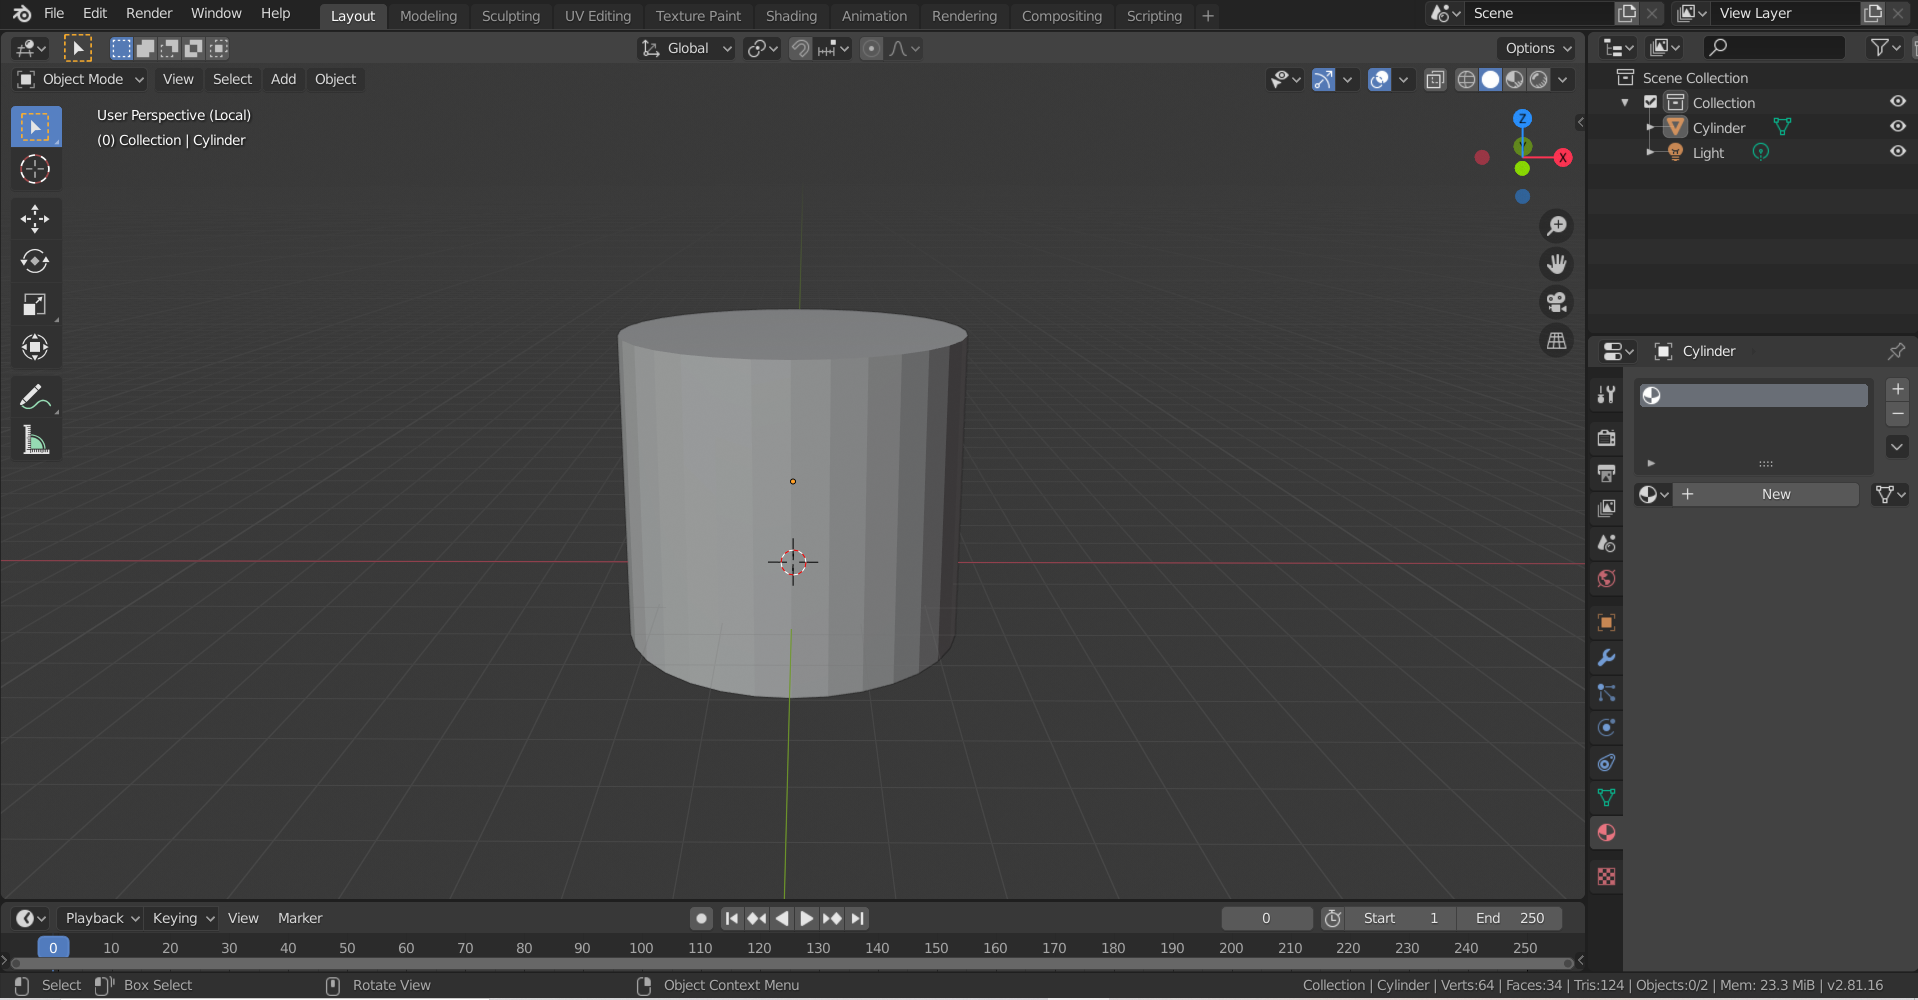
\includegraphics[scale=0.4]{Gambar/blender.png}
	\caption{Tampilan \textit{UI Blender} Blender versi 2.81}
	\label{fig:blender-ui}
\end{figure}

Bentuk silinder dipilih sebagai bentuk dari dunia VR karena permukaan samping dapat menampilkan pemandangan seperti di dunia nyata. Permukaan samping berbentuk persegi panjang, dan sifat melingkar dari permukaan dapat membuat menampilkan pemandangan di sekitar.

\section{Menampilkan \textit{StreetView API} pada Dunia VR}
Dengan menggunakan HTTP/HTTPS URL, gambar yang dihasilkan merupakan gambar persegi panjang saat menghadap satu arah sehingga tidak dapat secara langsung ditampilkan pada dunia VR ~\cite{streetview-api}. Untuk melakukannya, gambar dari empat arah harus digabungkan untuk menghasilkan pemandangan seperti  dunia nyata. Hal yang harus dilakukan untuk mencapai hal tersebut adalah menggabungkan gambar-gambar dari atribut \textit{heading} dari empat arah, dengan satu arah yang berlawanan dengan arah yang lain, lalu dua arah lain yang tegak lurus dengan arah pertama. Dengan kata lain, selisih setiap dua nilai \textit{heading} yang berurutan  bernilai 90 (misalnya \textit{heading} dengan nilai 0, 90, 180 dan 270). Gambar \ref{fig:comp-streetview} memperlihatkan empat gambar \textit{StreetView} dengan berbagai macam \textit{StreetView} dengan syarat tersebut.

\begin{figure}[]
	\begin{subfigure}{.5\textwidth}
  		\centering
  		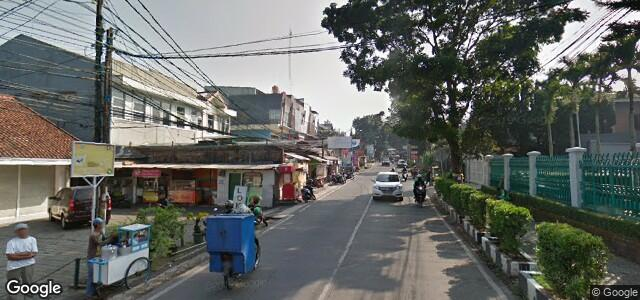
\includegraphics[width=1\linewidth]{Gambar/streetview0.png}
  		\caption{\textit{heading}=0}
  		\label{fig:streetview0}
	\end{subfigure}
	\begin{subfigure}{.5\textwidth}
  		\centering
  		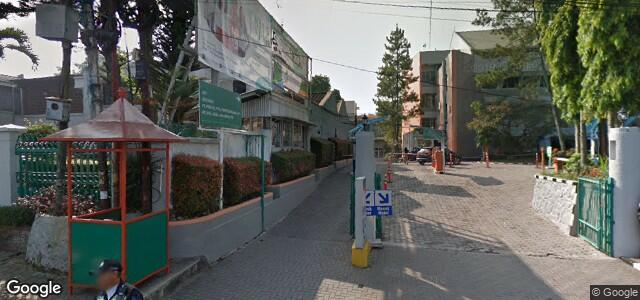
\includegraphics[width=1\linewidth]{Gambar/streetview90.png}
  		\caption{\textit{heading}=90}
  		\label{fig:streetview90}
	\end{subfigure}
	\begin{subfigure}{.5\textwidth}
  		\centering
  		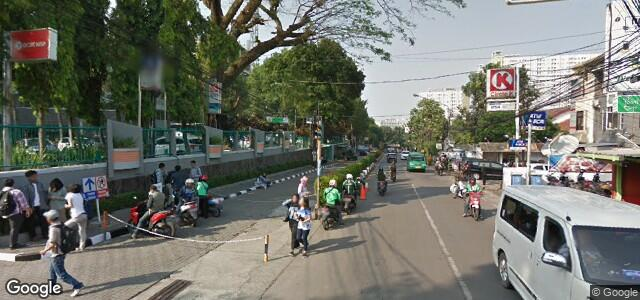
\includegraphics[width=1\linewidth]{Gambar/streetview180.png}
  		\caption{\textit{heading}=180}
  		\label{fig:streetview180}
	\end{subfigure}
	\begin{subfigure}{.5\textwidth}
  		\centering
  		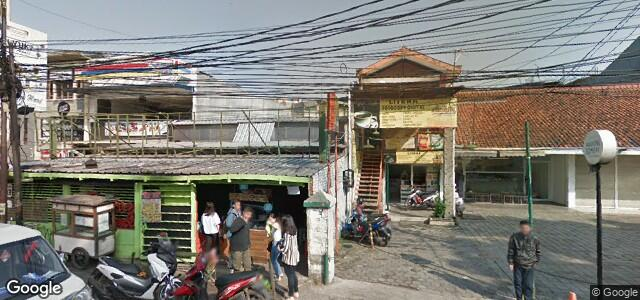
\includegraphics[width=1\linewidth]{Gambar/streetview270.png}
  		\caption{\textit{heading}=270}
  		\label{fig:streetview270}
	\end{subfigure}
	\caption{Pemanggilan \textit{StreetView API} yang berhasil, dengan \textit{URL} \url{https://maps.googleapis.com/maps/api/streetview?size=600x300\&location=-6.8746537,107.6046282\&key=(disamarkan)}, dengan parameter \textit{heading} yang berbeda-beda-jelaskan di bab 2 tentang keluaran directions.}
\label{fig:comp-streetview}
\end{figure}

Setelah mendapatkan gambar \textit{StreetView} dari semua arah, gambar-gagmbar tersebut digabungkan sehingga membentuk pemandangan seperti ada di lokasi tersebut. Gambar \ref{fig:streetview-vr} menunjukkan hasil penggabungan empat gambar dengan deskripsi di atas.

\begin{figure}[h]
	\centering
		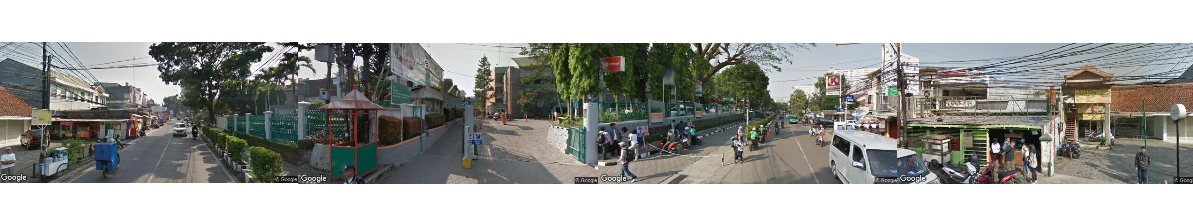
\includegraphics[width=6.5in,height=3in]{Gambar/connected_streetview.png}
	\caption{Contoh hasil penggabungan empat gambar \textit{StreetView}}
	\label{fig:streetview-vr}
\end{figure}

Setelah mendapatkan gambar \textit{StreetView} yang sudah digabungkan tersebut, gambar tersebut dapat dimanfaatkan sebagai tekstur untuk ruang pada \textit{file} OBJ yang berbentuk silinder sehingga pemandangan \textit{StreetView} dapat ditampilkan pada dunia VR.

\section{Integrasi dengan \textit{Directions API}}
Untuk mendapatkan rute perjalanan, \textit{Directions API} dapat dimanfaatkan ~\cite{directions-api}. \textit{File} yang diperoleh lewat \textit{Directions API} adalah \textit{file} JSON yang memiliki \textit{key} dan \textit{value}. Ada beberapa atribut (\textit{key}) dengan nilai (\textit{value}) yang ada pada \textit{file} JSON dari hasil pemanggilan \textit{Directions API} yang dapat dimanfaatkan.

\subsection{Menentukan Atribut yang Bermanfaat}
\textit{File} JSON yang dihasilkan memiliki beberapa tingkat \textit{key} dan \textit{value}. Pada tingkat pertama, ada tiga \textit{key}: \textit{geocoded\_waypoints}, \textit{status} dan \textit{routes}. \textit{Key} yang dapat digunakan adalah \textit{routes} yang menunjukkan jalan yang akan ditempuh. Pada tingkat berikutnya, \textit{key routes} memiliki \textit{value} seperti \textit{bounds}, \textit{copyrights}, dan \textit{legs}. Jika melihat bagian \textit{legs} yang menampung atribut-atribut jalan yang ditempuh, ada {\it distance}, {\it duration}, {\it end\_location}, {\it html\_instructions}, {\it maneuver}, {\it polyline}, {\it start\_location}, dan \textit{travel\_mode}. Dari beberapa atribut dari \textit{legs}, yang dapat digunakan adalah \textit{end\_location} dan \textit{start\_location}, yang menunjuk kepada posisi garis lintang dan garis bujur titik ujung dari jalan yang sedang ditempuh. 

\subsection{Cara Memanfaatkan Atribut}
\label{subs:directions-attr-use}
Setelah memperoleh nilai \textit{end\_location} dan \textit{start\_location}, jalur tempuh pada jalan yang sedang ditempuh dapat ditentukan lewat posisi garis lintang dan garis bujur kedua titik ujung jalan. Cara untuk membentuk jalan secara matematis adalah menggunakan selisih antara garis lintang dan garis bujur satu titik ujung jalan ke titik ujung jalan lain. 

%\subsubsection{Bresenhan's algorithm / DDA}
%https://www.geeksforgeeks.org/bresenhams-line-generation-algorithm/
%\subsubsection{Haversine Formula}
%https://www.geeksforgeeks.org/haversine-formula-to-find-distance-between-two-points-on-a-sphere/

\section{Cara Memanfaatkan \textit{Step Detector} Sensor}
Untuk membuat animasi atau perubahan pemandangan sesuai rute tempuh yang sudah diperoleh, harus ada perubahan gambar sesuai langkah kaki yang diambil pengguna. Jadi, setiap kali sensor mendapat rangsang, \textit{event} yang dipicu agar terjadi adalah gambar berubah seperti yang dijelaskan pada Subbab \ref{subs:directions-attr-use}, tetapi perubahan gambar \textit{StreetView} yang sesuai \textit{Directions API} harus berubah dengan tahap yang benar agar animasi pemandangan terlihat mulus.